\subsubsection{Analyzing fingerprinting API presence in Chrome and
  Firefox}

Recall that one of the key research questions we asked at the beginning of
this paper was if popular browsers such as Firefox and Chrome are
generally becoming more fingerprintable over time. In particular, we
were also interested in answering if every browser version is unique
in a fingerprintability sense.

Using the fingerprinting APIs that we collected (and described in
Section \ref{sec:methodology}), we aimed to determine how many of
these APIs are available and active in specific browser versions. That
is, we iterated through all the major Firefox and Chrome browser
versions between 2016 and 2020, and tested their fingerprintability.

In Chrome 49 (i.e., the oldest Chrome version in our analysis),
there existed 139 APIs from the suspicious fingerprinting APIs list. Which
means they could be used for fingerprinting. In Chrome
81 (the newest Chrome version in our analysis), there
existed 274 APIs from the suspicious fingerprinting APIs list. In short, the
number of APIs that could be used for fingerprinting Chrome versions
were increasing over time. That is, the data suggest that Chrome is
becoming easier to fingerprint.

Compared to Chrome, Firefox 45 (i.e., the oldest version in our study)
has 147 APIs from the suspicious fingerprinting APIs list. In constrast,
Firefox 75 (which is the latest Firefox version in our study) has 271
fingerprinting APIs from the suspicious fingerprinting APIs list.
Interestingly, though, Firefox 71 has 276 APIs from the suspicious
fingerprinting APIs list. Our data analysis suggests that
Firefox has become more fingerprintable over time, but that lately,
although more features are added to it, its fingerprintability might
have started to decline. In fact, Firefox has indeed started to take
the fingerprinting problem seriously and has been increasingly taking
steps to prevent it (e.g.,~\cite{FirefoxFingerprinting}).

Figure \ref{fig:fingerprint-apis} depicts, in detail, the presence of
fingerprinting APIs in Chrome and Firefox that we measured. Note that
in January 2017, there is a significant increase in the number of
fingerprinting APIs that each browser supports. More than 100
fingerprinting APIs were added to both browsers. To determine what
caused this spike, we investigated and analyzed the release notes of
both Firefox 51~\cite{firefox-51-notes} and Chrome
56~\cite{chrome-56-notes}.

The release notes indicate that HTML5 was enabled for all users by
default in Chrome 56. As of this version, Adobe Flash Player was
disabled and only allowed to run with specific user permissions.
Chrome also enabled the WebGL 2.0 API that provides a new rendering
context, and supports objects for the HTML5 Canvas elements. This
context allows rendering using an API that conforms closely to the
OpenGL ES 3.0
API~\footnote{https://www.khronos.org/registry/webgl/specs/latest/2.0/}.
Similarly, in Firefox 51, we observed that the browser had also added
WebGL2 support during that time.

When we analyzed our fingerprinting API list, we saw that the 107 new
fingerprinting APIs that became possible as of this date were actually
related to \texttt{WebGL2RenderingContext} which was added to Firefox
51 and Chrome 56. The straight-forward lesson to distill from our
observation is that browser vendors need to be extra careful when they
implement and release new features if they are interested in making
their browsers more difficult to fingerprint.

\begin{figure}[ht]
    \centering
    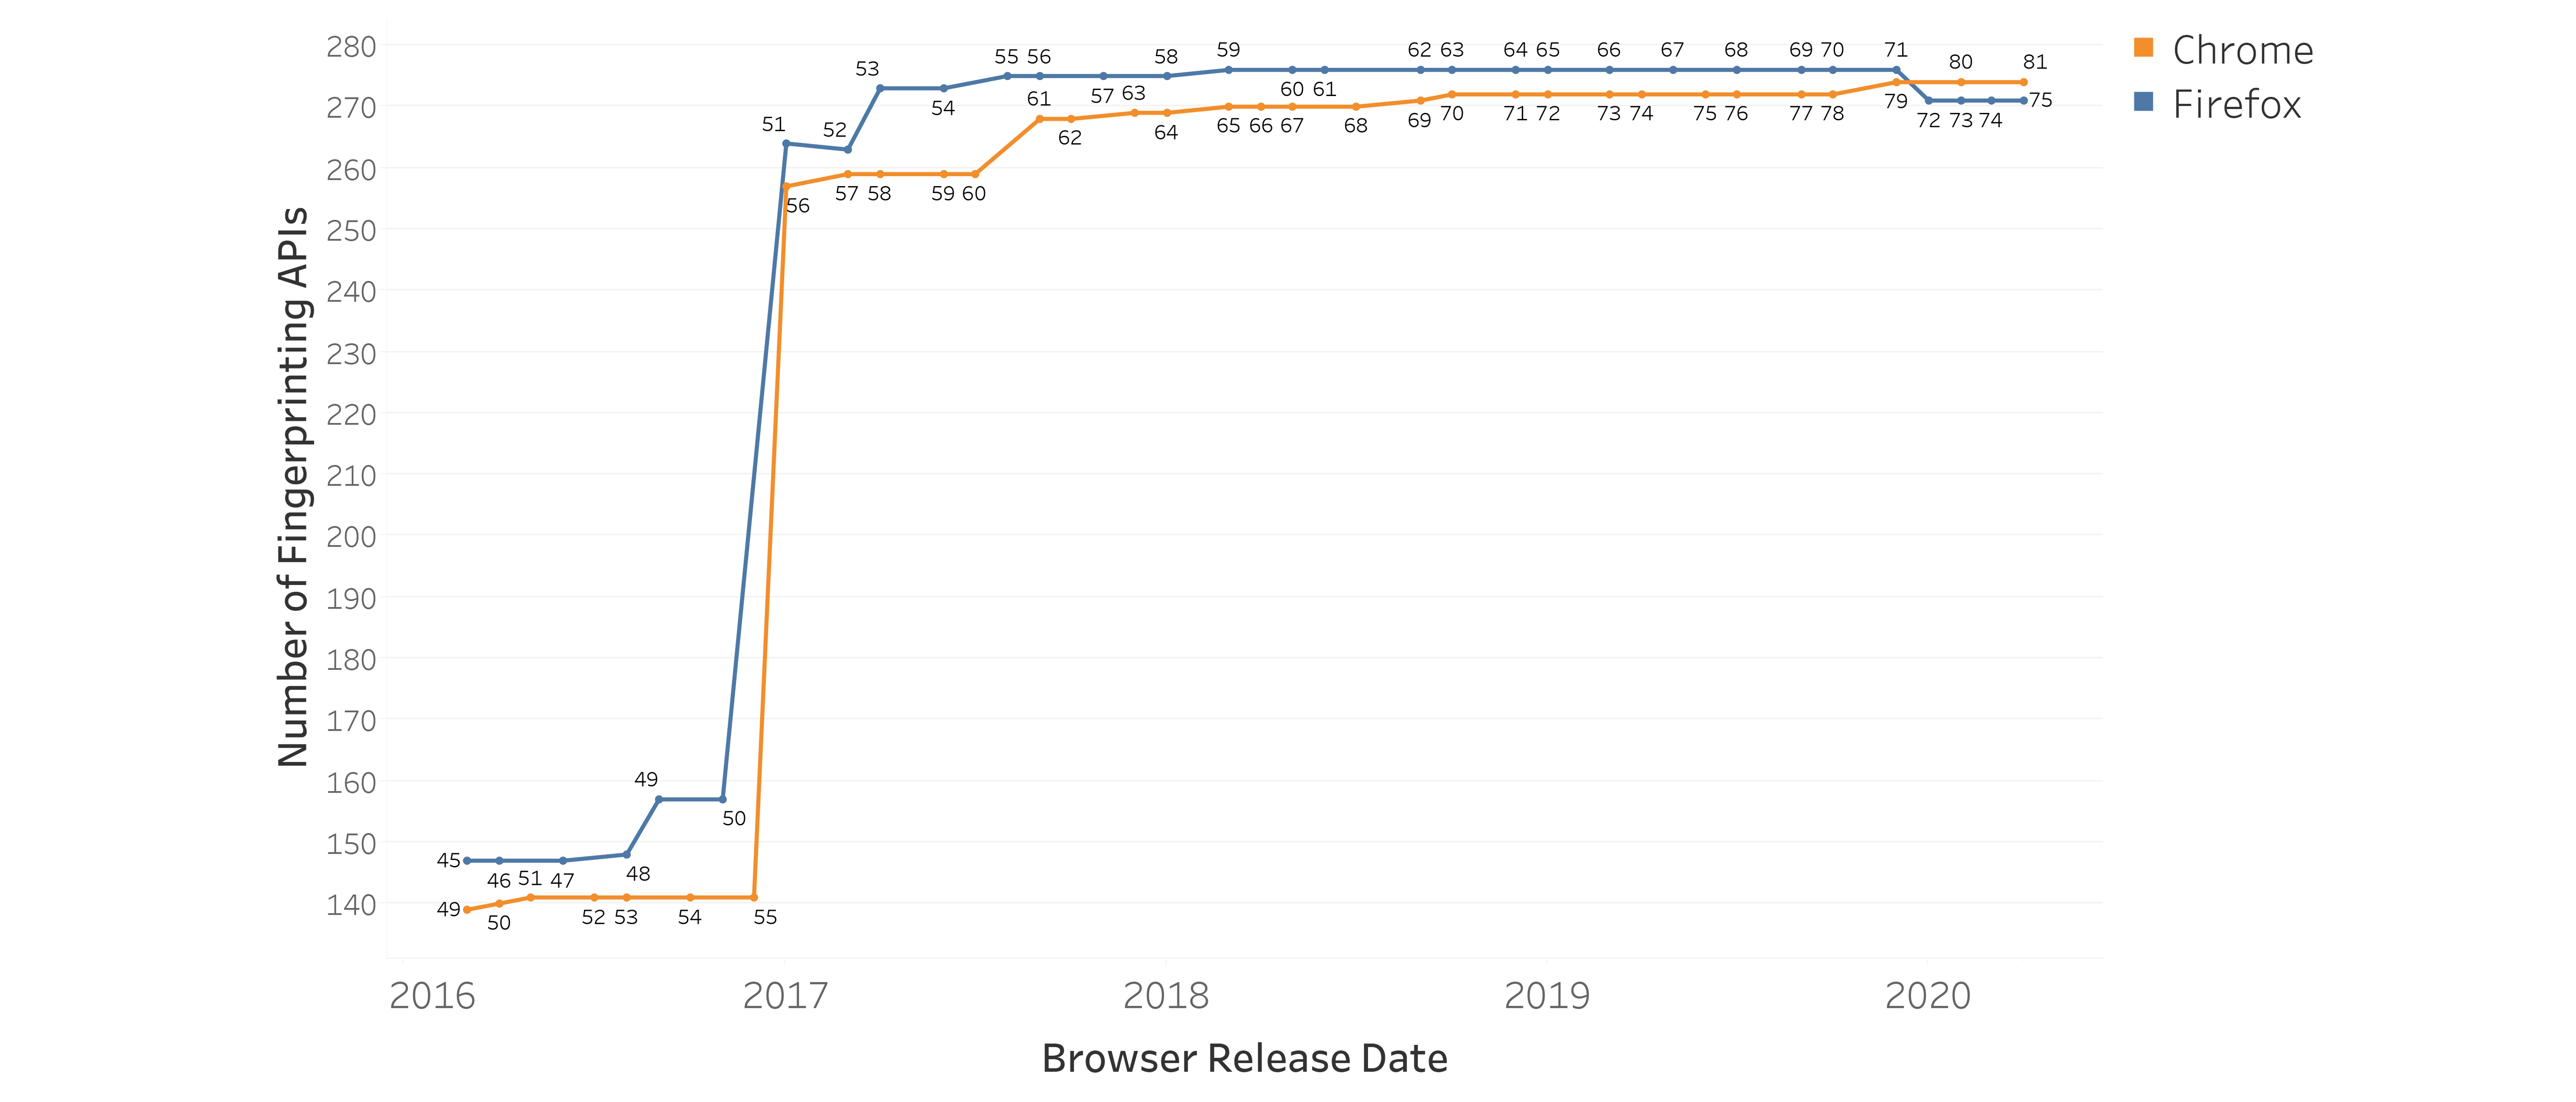
\includegraphics[width=\columnwidth]{figures/Fingerprinting-APIs.png}
    \caption{Presence of Fingerprinting APIs in Chrome and Firefox.}
    \label{fig:fingerprint-apis}
\end{figure}

We also collected the feature set for Google Chrome's Incognito mode
and also Firefox's Private Window mode in the corresponding browser versions
in our data gathering part to measure the fingerprintability of these browsers
while using these modes.
We found out that there is a small difference between the total number of features in the
regular mode versus the total number of features in the Incognito mode. 
For instance, Chrome 80's regular mode has 11946 features while it has 11936 features
in Incognito mode. We could say the same for Firefox's regular mode versus its Private Window Mode too.  
For example, Firefox 75's regular mode has 6370 total features while its Private Widnow Mode has 6358 features.
This was predictable since there are some features disabled in Incognito mode soo the number of available JS APIs
should be less than the regular mode.

After analysing the feature sets between these two modes, we focus on the difference 
in fingerprintability between regular mode and Incognito mode.
Surprisingly, for each Chrome version, all features that appear in the suspicious fingerprinting
APIs list in regular mode also appear in its Incognito mode's suspicious fingerprinting APIs.
The same happens in Firefox too. The fingerprinting APIs existing in a Firefox version's regular mode and private
window mode are identical. Thus we could conclude that Incognito mode and
private window mode do not help users against browser fingerprinting since every fingerprinting API that exists in
a version's normal mode, also appears in the same browser version's Incognito (or Private Window) mode.


\subsubsection{Unique Feature Set}

In our analyses, we automatically deduced a ``feature set'' for each
browser version that we analyzed. A feature set is a set of (i.e., the
list of) browser features that exist in that specific browser version
under analysis. When we compared the features sets for each browser
version to each other (e.g., Firefox 54 versus 55), we observed that
each feature set was unique for all the browser versions that we
tested. That is, there exist no two browsers that possess the same
feature set. Hence, from this observation, we can deduce that all the
browser versions that we analyzed are uniquely fingerprintable.

The reason why the feature sets are unique among different browser
versions is that each browser, as we described before, have recurring
as well as non-persistent features. As a result, the fact that vendors
continuously add, remove, and sometimes re-add features into their
browsers also make them more fingerprintable.

%One key difference between Google Chrome when compared to Mozilla
%Firefox is that Chrome is adding many more new features to the newer
%versions of the browser while at the same time keeping older features
%around. Firefox, in comparison, seems to be more aggressive with
%respect to removing older features from the browser, and hence,
%``debloating'' the software.

One interesting trend is that the differences between the feature sets
of Chrome and Firefox in their newer versions is becoming smaller.
That is, we observed much more intersections with each other than in
older versions. Our data suggest that the feature sets for both
Firefox and Chrome are converging towards homogeneity of browser
features.
